\documentclass[]{exam}
\usepackage{lmodern}
\usepackage{amssymb,amsmath}
\usepackage{ifxetex,ifluatex}
\usepackage{fixltx2e} % provides \textsubscript
\ifnum 0\ifxetex 1\fi\ifluatex 1\fi=0 % if pdftex
  \usepackage[T1]{fontenc}
  \usepackage[utf8]{inputenc}
\else % if luatex or xelatex
  \ifxetex
    \usepackage{mathspec}
    \makeatletter % undo the wrong changes made by mathspec
    \let\RequirePackage\original@RequirePackage
    \let\usepackage\RequirePackage
    \makeatother
  \else
    \usepackage{fontspec}
  \fi
  \defaultfontfeatures{Ligatures=TeX,Scale=MatchLowercase}
\fi
% use upquote if available, for straight quotes in verbatim environments
\IfFileExists{upquote.sty}{\usepackage{upquote}}{}
% use microtype if available
\IfFileExists{microtype.sty}{%
\usepackage{microtype}
\UseMicrotypeSet[protrusion]{basicmath} % disable protrusion for tt fonts
}{}
\usepackage{hyperref}
\hypersetup{unicode=true,
            pdftitle={Homework 2},
            pdfborder={0 0 0},
            breaklinks=true}
\urlstyle{same}  % don't use monospace font for urls
\IfFileExists{parskip.sty}{%
\usepackage{parskip}
}{% else
\setlength{\parindent}{0pt}
\setlength{\parskip}{6pt plus 2pt minus 1pt}
}
\setlength{\emergencystretch}{3em}  % prevent overfull lines
\providecommand{\tightlist}{%
  \setlength{\itemsep}{0pt}\setlength{\parskip}{0pt}}
\setcounter{secnumdepth}{0}
% Redefines (sub)paragraphs to behave more like sections
\ifx\paragraph\undefined\else
\let\oldparagraph\paragraph
\renewcommand{\paragraph}[1]{\oldparagraph{#1}\mbox{}}
\fi
\ifx\subparagraph\undefined\else
\let\oldsubparagraph\subparagraph
\renewcommand{\subparagraph}[1]{\oldsubparagraph{#1}\mbox{}}
\fi

\usepackage{booktabs}

\title{Homework 2}

\usepackage[margin=.75in]{geometry}
\RequirePackage{amsmath}
\usepackage{amssymb}
\usepackage{textcase}
\usepackage{soul}
\usepackage{indentfirst}

\newcommand{\eps}{\varepsilon}
\newcommand{\kron}{\otimes}
\DeclareMathOperator{\diag}{diag}
\DeclareMathOperator{\trace}{trace}
\DeclareMathOperator{\tvec}{vec}
\DeclareMathOperator{\rank}{rank}
\DeclareMathOperator{\tspan}{span}
\DeclareMathOperator*{\minimize}{minimize}
\DeclareMathOperator*{\maximize}{maximize}
\DeclareMathOperator{\subjectto}{subject\ to}

\newcommand{\mat}[1]{\boldsymbol{#1}}
\renewcommand{\vec}[1]{\boldsymbol{\mathrm{#1}}}
\newcommand{\vecalt}[1]{\boldsymbol{#1}}

\newcommand{\conj}[1]{\overline{#1}}

\newcommand{\normof}[1]{\|#1\|}
\newcommand{\onormof}[2]{\|#1\|_{#2}}

\newcommand{\MIN}[2]{\begin{array}{ll} \displaystyle \minimize_{#1} & {#2} \end{array}}
\newcommand{\MINone}[3]{\begin{array}{ll} \displaystyle \minimize_{#1} & {#2} \\ \subjectto & {#3} \end{array}}
\newcommand{\OPTone}{\MINone}
\newcommand{\MINthree}[5]{\begin{array}{ll} \displaystyle \minimize_{#1} & {#2} \\ \subjectto & {#3} \\ & {#4} \\ & {#5} \end{array}}

\newcommand{\MAX}[2]{\begin{array}{ll} \displaystyle \maximize_{#1} & {#2} \end{array}}
\newcommand{\MAXone}[3]{\begin{array}{ll} \displaystyle \maximize_{#1} & {#2} \\ \subjectto & {#3} \end{array}}


\newcommand{\itr}[2]{#1^{(#2)}}
\newcommand{\itn}[1]{^{(#1)}}

\newcommand{\prob}{\mathbb{P}}
\newcommand{\probof}[1]{\prob\left\{ #1 \right\}}

\newcommand{\pmat}[1]{\begin{pmatrix} #1 \end{pmatrix}}
\newcommand{\bmat}[1]{\begin{bmatrix} #1 \end{bmatrix}}
\newcommand{\spmat}[1]{\left(\begin{smallmatrix} #1 \end{smallmatrix}\right)}
\newcommand{\sbmat}[1]{\left[\begin{smallmatrix} #1 \end{smallmatrix}\right]}

\newcommand{\RR}{\mathbb{R}}
\newcommand{\CC}{\mathbb{C}}

\providecommand{\eye}{\mat{I}}
\providecommand{\mA}{\ensuremath{\mat{A}}}
\providecommand{\mB}{\ensuremath{\mat{B}}}
\providecommand{\mC}{\ensuremath{\mat{C}}}
\providecommand{\mD}{\ensuremath{\mat{D}}}
\providecommand{\mE}{\ensuremath{\mat{E}}}
\providecommand{\mF}{\ensuremath{\mat{F}}}
\providecommand{\mG}{\ensuremath{\mat{G}}}
\providecommand{\mH}{\ensuremath{\mat{H}}}
\providecommand{\mI}{\ensuremath{\mat{I}}}
\providecommand{\mJ}{\ensuremath{\mat{J}}}
\providecommand{\mK}{\ensuremath{\mat{K}}}
\providecommand{\mL}{\ensuremath{\mat{L}}}
\providecommand{\mM}{\ensuremath{\mat{M}}}
\providecommand{\mN}{\ensuremath{\mat{N}}}
\providecommand{\mO}{\ensuremath{\mat{O}}}
\providecommand{\mP}{\ensuremath{\mat{P}}}
\providecommand{\mQ}{\ensuremath{\mat{Q}}}
\providecommand{\mR}{\ensuremath{\mat{R}}}
\providecommand{\mS}{\ensuremath{\mat{S}}}
\providecommand{\mT}{\ensuremath{\mat{T}}}
\providecommand{\mU}{\ensuremath{\mat{U}}}
\providecommand{\mV}{\ensuremath{\mat{V}}}
\providecommand{\mW}{\ensuremath{\mat{W}}}
\providecommand{\mX}{\ensuremath{\mat{X}}}
\providecommand{\mY}{\ensuremath{\mat{Y}}}
\providecommand{\mZ}{\ensuremath{\mat{Z}}}
\providecommand{\mLambda}{\ensuremath{\mat{\Lambda}}}
\providecommand{\mSigma}{\ensuremath{\mat{\Sigma}}}
\providecommand{\mPbar}{\bar{\mP}}

\providecommand{\ones}{\vec{e}}
\providecommand{\va}{\ensuremath{\vec{a}}}
\providecommand{\vb}{\ensuremath{\vec{b}}}
\providecommand{\vc}{\ensuremath{\vec{c}}}
\providecommand{\vd}{\ensuremath{\vec{d}}}
\providecommand{\ve}{\ensuremath{\vec{e}}}
\providecommand{\vf}{\ensuremath{\vec{f}}}
\providecommand{\vg}{\ensuremath{\vec{g}}}
\providecommand{\vh}{\ensuremath{\vec{h}}}
\providecommand{\vi}{\ensuremath{\vec{i}}}
\providecommand{\vj}{\ensuremath{\vec{j}}}
\providecommand{\vk}{\ensuremath{\vec{k}}}
\providecommand{\vl}{\ensuremath{\vec{l}}}
\providecommand{\vm}{\ensuremath{\vec{m}}}
\providecommand{\vn}{\ensuremath{\vec{n}}}
\providecommand{\vo}{\ensuremath{\vec{o}}}
\providecommand{\vp}{\ensuremath{\vec{p}}}
\providecommand{\vq}{\ensuremath{\vec{q}}}
\providecommand{\vr}{\ensuremath{\vec{r}}}
\providecommand{\vs}{\ensuremath{\vec{s}}}
\providecommand{\vt}{\ensuremath{\vec{t}}}
\providecommand{\vu}{\ensuremath{\vec{u}}}
\providecommand{\vv}{\ensuremath{\vec{v}}}
\providecommand{\vw}{\ensuremath{\vec{w}}}
\providecommand{\vx}{\ensuremath{\vec{x}}}
\providecommand{\vy}{\ensuremath{\vec{y}}}
\providecommand{\vz}{\ensuremath{\vec{z}}}
\providecommand{\vpi}{\ensuremath{\vecalt{\pi}}}

\providecommand{\vlambda}{\ensuremath{\vecalt{\lambda}}}


\sodef\allcapsspacing{\upshape}{0.15em}{0.65em}{0.6em}%

\makeatletter
\def\maketitle{%
\par
\hrule height 0.75pt\vspace{1ex}
\par\noindent
\begin{minipage}{0.5\textwidth}
\scshape
purdue university $\cdot$ cs 51500 \\
matrix computations
\end{minipage}
\begin{minipage}{0.5\textwidth}
\raggedleft
\MakeTextUppercase{\allcapsspacing{\@title}}\\[0.2ex]
\textit{\@author}\\[0.2ex]
\textit{\@date}
\end{minipage}
\par\vspace{1ex}
\hrule height 1pt
\vspace{2ex}
\par
}
\makeatother

\author{Jinen Setpal}
\title{Lecture Notes}
% auto generate a title
% \AtBeginDocument{\maketitle}

\title{Homework 2 Submission}

% Question header formatting
\qformat{\hfill \textbf{Problem \thequestion} \hfill}

\DeclareMathOperator{\Tr}{Tr}
\DeclareMathOperator{\Cov}{Cov}
\DeclareMathOperator{\Concat}{Concat}
\DeclareMathOperator*{\argsup}{arg\,sup}
\DeclareMathOperator*{\arginf}{arg\,inf}
\DeclareMathOperator*{\argmax}{arg\,max}
\DeclareMathOperator*{\argmin}{arg\,min}
\DeclareMathOperator*{\indep}{\perp \!\!\! \perp}
\setcounter{MaxMatrixCols}{20}

\newcommand{\divider}{\line(1,0){\textwidth}}

\allowdisplaybreaks

% Package for enumerated lists using letters
\usepackage{enumitem}

% Algorithms
\usepackage{algpseudocode}
\usepackage{algorithm}
\usepackage{nicefrac}
\usepackage{graphicx}
\usepackage{fancyvrb,fvextra}
\usepackage[usenames,dvipsnames]{xcolor}
\usepackage{listings}
\usepackage{hyperref}

%%
%% Julia definition (c) 2014 Jubobs
%%
\lstdefinelanguage{Julia}%
  {morekeywords={abstract,break,case,catch,const,continue,do,else,elseif,%
      end,export,false,for,function,immutable,import,importall,if,in,%
      macro,module,otherwise,quote,return,switch,true,try,type,typealias,%
      using,while},%
   sensitive=true,%
   alsoother={\$},%
   morecomment=[l]\#,%
   morecomment=[n]{\#=}{=\#},%
   morestring=[s]{"}{"},%
   morestring=[m]{'}{'},%
}[keywords,comments,strings]%

\lstset{%
    language         = Julia,
    basicstyle       = \ttfamily,
    keywordstyle     = \bfseries\color{blue},
    stringstyle      = \color{magenta},
    commentstyle     = \color{ForestGreen},
	breaklines=true,
    showstringspaces = false,
}

\begin{document}
\maketitle

\hypertarget{problem-0-homework-checklist}{%
\subsection{Checklist}\label{problem-0-homework-checklist}}

\begin{enumerate}
	\item Cross-checked independent work with Kunal Kapur, brief discussion of approach with Diego Aguilar.
	\item No use of AI tools.
	\item Code is included!
\end{enumerate}

\begin{questions}

\question
\hfill

\begin{enumerate}[label=\arabic*.]
	\item Here's the approach:
		\begin{enumerate}[label=\alph*.]
			\item Copy HW1 Q7 to get Poisson's Equation as a linear system w/o boundary conditions for $n = 10$.
			\item Flip the signs and consider the equivalent problem: $\mA \vx = \vb \iff -\mA \vx = -\vb$
			\item Check if new $\mA' := -\mA$ is PD by diagonal dominance.
			\item Solve $\mA'$ with Richardson's Method ($\hat{\vx}$) setting $\alpha = 1$, and with Julia's solver ($\vx^*$) as the designated oracle. Then compare the difference in solutions (relative error): $\nicefrac{\|\hat{\vx} - \vx^* \|_2}{\| \vx^* \|}$
		\end{enumerate}

		\paragraph{Code}
			\begin{lstlisting}
using LinearAlgebra, SparseArrays, Plots

function map_index(i::Integer, j::Integer, n::Integer)
	if 1 < i < n+1 && 1 < j < n+1
		return 4n + (i - 2)*(n-1) + j-1
	elseif i == 1
		return j
	elseif i == n+1
		return n + 1 + j
	elseif j == 1
		return 2(n+1) + i - 1
	elseif j == n+1
		return 2(n+1) + n - 2 + i
	end
end

function laplacian(n::Integer, f::Function)
	A = sparse(1I, (n+1)^2, (n+1)^2)
	A[diagind(A)[4n+1:end]] .= -4

	fvec = zeros((n+1)^2)

	global row_index = 4n + 1
	for i in 2:n
		for j in 2:n
			A[row_index, map_index(i-1, j, n)] = 1
			A[row_index, map_index(i+1, j, n)] = 1
			A[row_index, map_index(i, j-1, n)] = 1
			A[row_index, map_index(i, j+1, n)] = 1
			fvec[row_index] = f(i, j)

			global row_index += 1
		end
	end

	return A, fvec/n^2
end
n = 10
A, fv = laplacian(n, (x, y) -> 1)

A = A[4n+1:end,4n+1:end]
fv = fv[4n+1:end]

# equivalent system of equations
A = -A
fv = -fv

# check if new A is PD
is_pd = all((2 .* Array(diag(A)) - sum(A, dims=2)) .>= 0)  # diagonally dominant implies PD
println("Is `A` definitely PD? ", is_pd)

alpha = 1
T = 100
oracle_sol = A\fv
norm_oracle_sol = norm(oracle_sol)

function richardson(A::SparseMatrixCSC, fv::Vector, T::Integer, alpha::Number, oracle_sol::Vector)
	norm_oracle_sol = norm(oracle_sol)
	x_hat = 1 * fv  # copy-by-value, not reference (https://stackoverflow.com/a/76109083/10671309)
	err = [norm(x_hat - oracle_sol) / norm_oracle_sol]   # initial error
	for itr in 1:T
		x_hat = (I - (alpha * A)) * x_hat + (alpha * fv)
		push!(err, norm(x_hat - oracle_sol) / norm_oracle_sol)
	end
	return (x_hat, err)
end

function richardson(A::SparseMatrixCSC, fv::Vector, T::Integer, alpha::Number)
	x_hat = 1 * fv  # copy-by-value, not reference (https://stackoverflow.com/a/76109083/10671309)
	res = [norm(A * x_hat - fv) / norm(fv)]
	for itr in 1:T
		x_hat = (I - (alpha * A)) * x_hat + (alpha * fv)
		push!(res, norm(A * x_hat - fv) / norm(fv))
	end
	return (x_hat, res, minimum(push!(findall(x->x < 1e-5, res), T+1)))
end

x_hat, err = richardson(A, fv, T, alpha, oracle_sol)
println(norm(x_hat - A\fv))
		\end{lstlisting}
		\paragraph{Output}
		\begin{lstlisting}
Is `A` definitely PD? true
8.294254291121953184390746064420433471290093240340010870951240578726456583749248e+78
		\end{lstlisting}
		Richardson's Method produces a solution that diverges dramatically as we iterate, with a final error reading $8.29 \cdot 10^{78}$. Even though y is $\log_{10}$-scale it increases sharply:
		\begin{center}
			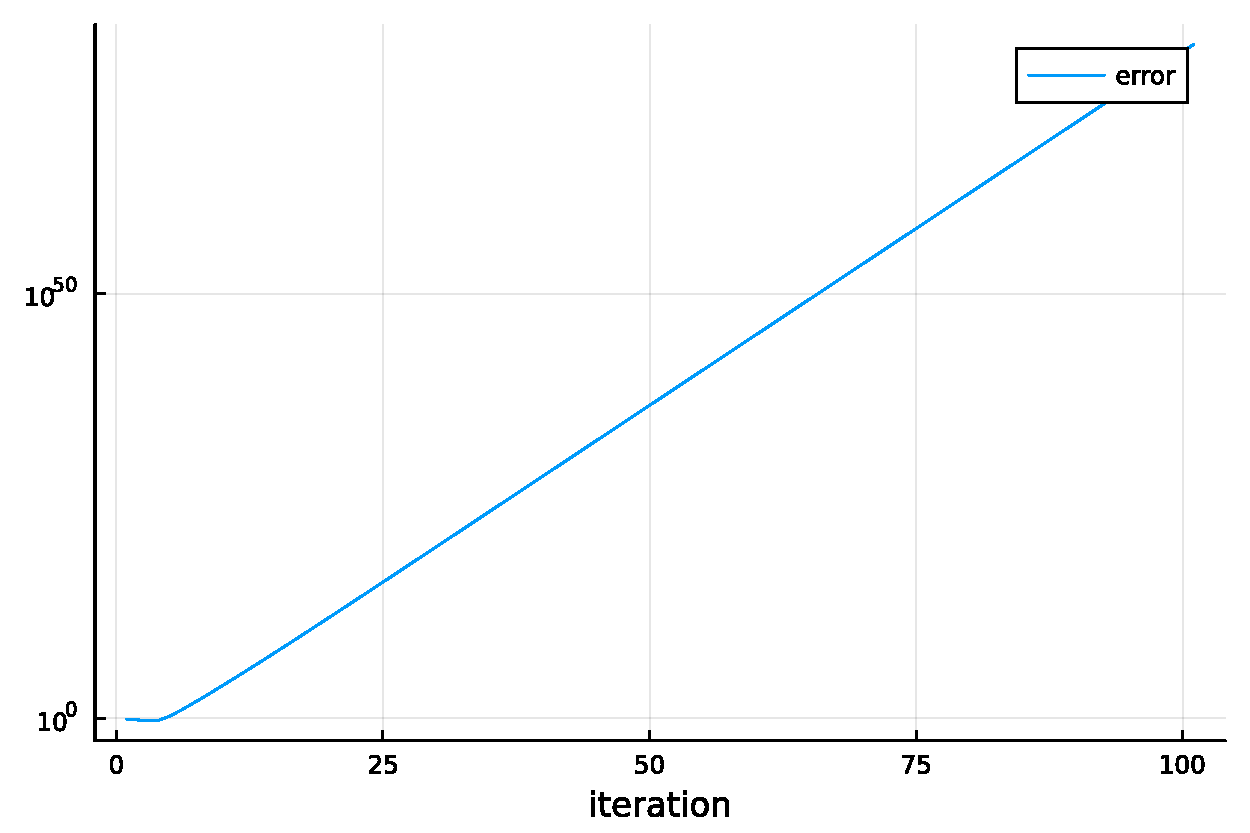
\includegraphics[width=.7\textwidth]{code/q1-1.pdf}
		\end{center}
		Setting $T = 1000$ we get a loss of \texttt{Inf} and at this point we can confidently claim that this method will not converge even as $T \rightarrow \infty$.
	\item We can try a simple grid search with $\alpha := c \cdot 10^p \quad \forall c \in \{1, 2, \ldots, 9\}, p \in \{-1, -2, \ldots, -5\}$:
		\paragraph{Code}
\begin{lstlisting}
alphs = []
errs = []
ress = []
tols = []
for alph_pow in 0:2
	for alph_coeff in 9:-.1:1
		local alpha = alph_coeff * 10^(-1. *alph_pow)
		local (x_hat, res, min_tol_iter) = richardson(A, fv, T, alpha)
		local err = norm(x_hat - oracle_sol) / norm_oracle_sol

		push!(alphs, alpha)
		push!(errs, err)
		push!(ress, res)
		push!(tols, min_tol_iter)
	end
end
		\end{lstlisting}
		\paragraph{Output}
		Here's the relative error progression:
		\begin{center}
			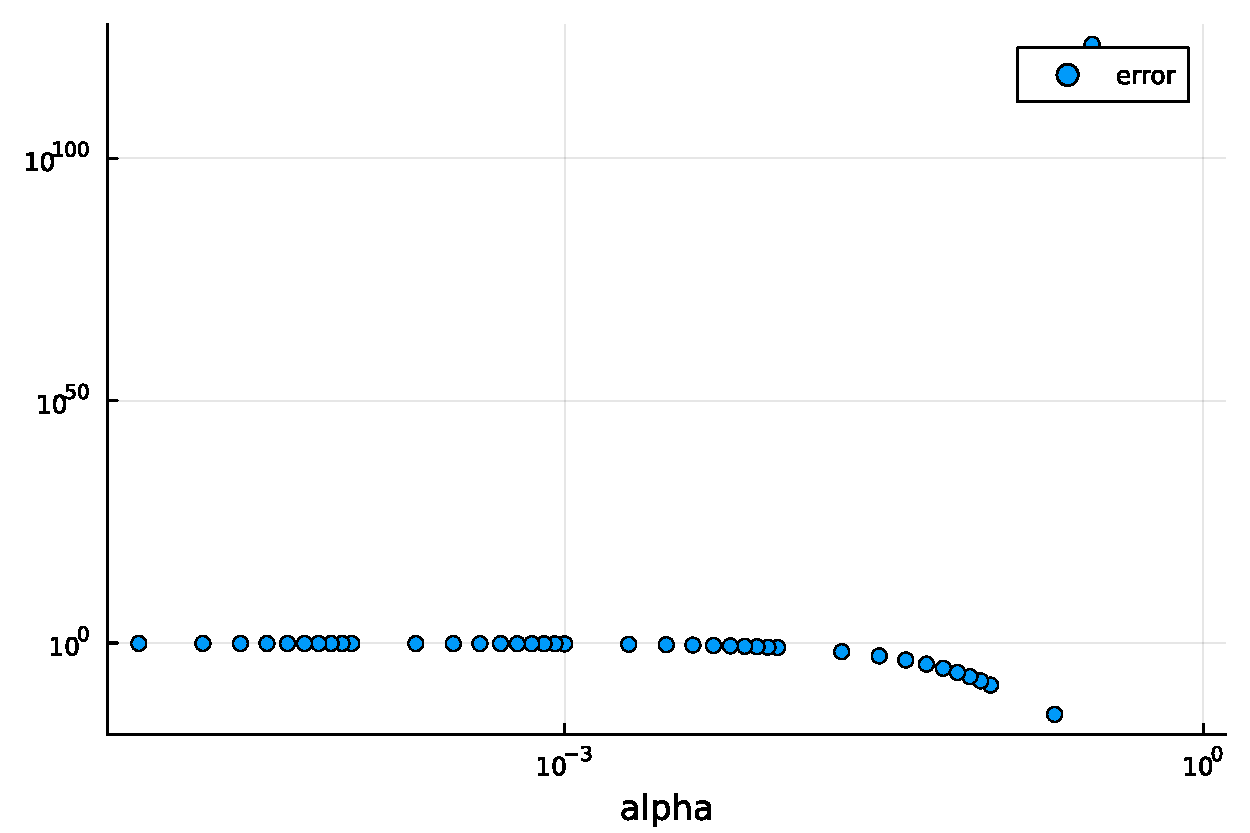
\includegraphics[width=.7\textwidth]{code/q1-2.pdf}
		\end{center}
		Picking the largest $\alpha$ with relative error $< 1$, we get $\alpha = 0.2$ as a feasible choice with relative error $0.014$ and relative residual $0.013$ for $T = 100$.
	\item Good news, with $n = 20$, we still have $\alpha = 0.2$ as a feasible solution. Bad news, the error is higher: relative error is $0.352$ and relative residual is $0.3$. I suspected I'm being too stingy with iterations so I set $T = 1000$ and now it is a more respectable relative error $= 4.75 \cdot 10^{-5}$ and relative residual $= 4.06 \cdot 10^{-5}$.
	\item Very informally, from the figure in part 2, error w.r.t.~$\alpha$ seems convex, and our previous feasible $\alpha = 0.2$ seems close to the minima, so I'll just do a more focused search around that:
		\paragraph{Code}
		\begin{lstlisting}
T = 1000

alphs = []
errs = []
ress = []
tols = []
for alph_pow in 0:2
	for alph_coeff in 9:-.1:1
		local alpha = alph_coeff * 10^(-1. *alph_pow)
		local (x_hat, res, min_tol_iter) = richardson(A, fv, T, alpha)
		local err = norm(x_hat - oracle_sol) / norm_oracle_sol

		push!(alphs, alpha)
		push!(errs, err)
		push!(ress, res)
		push!(tols, min_tol_iter)
	end
end

tol = 1e-5
largest_alpha = maximum(alphs[errs .< tol])
println("largest feasible alpha: ", largest_alpha)
println("relative error: ", errs[alphs .== largest_alpha][end])
println("relative residual: ", ress[alphs .== largest_alpha][end][end])
println("fastest alpha: ", alphs[findall(x-> x == minimum(tols), tols)][end])
		\end{lstlisting}
		\paragraph{Output}
		\begin{enumerate}[label=\alph*.]
			\item With $n = 10$:
				\begin{lstlisting}
largest feasible alpha: 0.25
relative error: 1.513596834021183337855890852231162135341721304455506905165879707855506594343833e-16
relative residual: 9.717969227135053e-16
fastest alpha: 0.25
				\end{lstlisting}
			\item With $n = 20$:
				\begin{lstlisting}
largest feasible alpha: 0.25
relative error: 3.943854431512536591214718270280764027830931906794095621191708359298462677555546e-06
relative residual: 3.3672320687686646e-6
fastest alpha: 0.25
				\end{lstlisting}
		\end{enumerate}
		In either case, $\alpha = 0.25$ converges the quickest.
	\item Reading $\alpha < 0.25$ is encouraging. We know that our method will converge for $\alpha < \nicefrac{2}{\rho(\mA)}$. T.P.T.
		\begin{gather*}
			\alpha < 0.25 \implies \alpha < \frac{2}{\rho(\mA)}
			\intertext{Or, equivalently:}
			\rho(\mA) \leq 8 \quad \mathrm{where} \quad
			\rho(\mA) = \max \{ |\lambda| : \mA \vx = \lambda \vx, \quad \vx \in \mathbb{R}^n \setminus \mathbf{0}_n \}
		\end{gather*}
		We can massage the eigenvector definition a bit:
		\begin{align*}
			\mA \vx = \lambda \vx &\implies \| \mA \vx \| = \| \lambda \vx \| \\
			&\implies \| \mA \vx \| = |\lambda| \| \vx \| \\
			&\implies |\lambda| = \frac{\| \mA \vx \|}{\| \vx \|} \leq \frac{\| \mA \| \| \vx \|}{\| \vx \|} = \| \mA \|
		\end{align*}
		Importantly, we need our choice of matrix norm to be submultiplicative for the last step.
		$\therefore |\lambda| < \|\mA\|~\forall \lambda$, which further implies $\rho(\mA) < \| \mA \|$. We choose $\| \cdot \|_{\infty}$ as the norm; in addition to being submultiplicative, this is very important because we know the structure of $\mA$: each row is sparse and has one $4$ and {\it at-most four} $-1$'s. Picking the largest possible absolute case allows us to calculate $\|A\|_{\infty} = \max^m_{i=1} \sum^n_{j=1} |\mA_{ij}| = 8$.
		\begin{gather*}
			\therefore \rho(\mA) \leq \| \mA \|_{\infty} = 8
		\end{gather*}
		Which satisfies the desired property, proving that $\alpha < 0.25$ will converge for any $n \in \mathbb{N}$.
\end{enumerate}

\newpage
\question
\hfill


\begin{enumerate}[label=\arabic*.]
	\item We have:
		\begin{gather*}
			f(\mA) = \max_{i,j} | \mA_{i,j}| = \max_{i} | vec(\mA)_i| = \| vec(\mA) \|_{\infty}
		\end{gather*}
		$f$ is the well-known max norm, with just an extra `flatten' step added to the input.
	\item T.P.T:
		\begin{equation*}
			\exists \mA \in \mathbb{R}^{m \times n},~\vx \in \mathbb{R}^{n} : f(\mA \vx) > f(\mA) f(\vx)
		\end{equation*}
		Proof by example:
		\begin{gather*}
			\mathrm{Let} \quad \mA = \bmat{1 & 1 \\ 1 & 1}, \quad \vx = \bmat{1 & 1}^T
		\end{gather*}
		Then, we have:
		\begin{gather*}
			f(\mA \vx) = f\left(\bmat{1 & 1 \\ 1 & 1} \bmat{1 & 1}^T \right) = f\left( \bmat{2 & 2}^T \right) = \max \{2, 2\} = 2 \\
			f(\mA) f(\vx) = f\left(\bmat{1 & 1 \\ 1 & 1}\right) f \left(\bmat{1 & 1}^T \right) = \max \{1, 1, 1, 1\} \cdot \max\{1, 1\} = 1 \cdot 1 = 1 \\
			f(\mA) f(\vx) = 1 < 2 = f(\mA \vx) \implies f(\mA) f(\vx) < f(\mA \vx)
		\end{gather*}
	\item Simplifying $\sigma$, T.P.T.
		\begin{gather*}
			\exists \sigma > 0: f(\mA \vx) \leq \sigma f(\mA) f(\vx) \qquad \forall \mA \in \mathbb{R}^{m \times n},~\vx \in \mathbb{R}^m,~m, n \in \mathbb{N}
		\end{gather*}
		We have:
		\begin{align*}
			f(\mA \vx) &= \max_{i} \left| \sum^{n}_{j=1} \mA_{i,j} \vx_j \right| \\
			&\leq \max_{i} \left| \sum^{n}_{j=1} |\mA_{i,j}| |\vx_j| \right| \\
			\intertext{All summands are positvie, so we can drop the outer absolute:}
			&= \max_{i} \sum^{n}_{j=1} |\mA_{i,j}| |\vx_j| \\
			&\leq \max_{i} \sum^{n}_{j=1} \max_{k,l}|\mA_{k,l}| \max_k|\vx_k| \\
			&= \max_{i} \sum^{n}_{j=1} f(\mA) f(\vx) \\
			\intertext{$i$ has no role to play in this equation, we can drop the max:}
			&= \sum^{n}_{j=1} f(\mA) f(\vx) \\
			&= n \cdot f(\mA) f(\vx) \\
			f(\mA \vx) &\leq n \cdot f(\mA) f(\vx)
		\end{align*}
		Since $n > 0,$ we can set $\sigma := n$ which gives us the desired sub-multiplicativity.
\end{enumerate}

\newpage
\question
\hfill

\begin{enumerate}[label=\arabic*.]
	\item T.P.T:
		\begin{align*}
			\forall \eps > 0,~\alpha_p \in (0, 1) \quad \exists \alpha_r \in (0, 1): \limsup_{k \rightarrow \infty} \| (\mI - \alpha_p \mP) \vx^{(k)} - (1 - \alpha_p) \vv \| < \eps \\
			\mathrm{where} \quad \vx^{(k)} := (\mI - \alpha_r(\mI - \alpha_p \mP)) \vx^{(k - 1)} + \alpha_r (1 - \alpha_p) \vv
		\end{align*}
		Let's first inspect the evolution of the residual:
		\begin{align*}
			(\mI - \alpha_p \mP) \vx^{(k)} - (1 - \alpha_p) \vv
			&= (\mI - \alpha_p \mP) (\mI - \alpha_r(\mI - \alpha_p \mP)) \vx^{(k - 1)} + \alpha_r (1 - \alpha_p) \vv - (1 - \alpha_p) \vv \\
			&= \left(\mI - \alpha_r(\mI - \alpha_p \mP) - \alpha_p \mP + \alpha_p^2 \alpha_r \mP^2 \right) \vx^{(k - 1)} + \alpha_r (1 - \alpha_p) \vv - (1 - \alpha_p) \vv \\
			&= \left(\mI - \alpha_p \mP \right) \vx^{(k - 1)}  - (1 - \alpha_p) \vv + \left(\alpha_p^2 \alpha_r \mP^2 - \alpha_r(\mI - \alpha_p \mP) \right) \vx^{(k - 1)} + \alpha_r (1 - \alpha_p) \vv \\
			&= \left(\mI - \alpha_p \mP \right) \vx^{(k - 1)}  - (1 - \alpha_p) \vv + \left(\alpha_p^2 \alpha_r \mP^2 - \alpha_r \alpha_p \mP  + \alpha_r \mI \right) \vx^{(k-1)} + \alpha_r (1 - \alpha_p) \vv \\
			&= \left(\mI - \alpha_p \mP \right) \vx^{(k - 1)}  - (1 - \alpha_p) \vv + \alpha_r \left( \left(\alpha_p^2 \mP^2 - \alpha_p \mP + \mI \right) \vx^{(k-1)} + (1 - \alpha_p) \vv \right) \\
			&= \left(\mI - \alpha_p \mP \right) \vx^{(k - 1)}  - (1 - \alpha_p) \vv + \alpha_r \alpha_p^2 \mP^2 \vx^{(k-1)} - \alpha_r \left( \left(\mI - \alpha_p \mP \right) \vx^{(k-1)} - (1 - \alpha_p) \vv \right) \\
			\intertext{Let $\vr^{(k)}$ be the residual at step $k$. Then, we have:}
			 \vr^{(k)} &= \vr^{(k - 1)} + \alpha_r \alpha_p^2 \mP^2 \vx^{(k-1)} - \alpha_r \vr^{(k - 1)} = (1 - \alpha_r) \vr^{(k - 1)} + \alpha_r \alpha_p^2 \mP^2 \vx^{(k-1)} \tag{1}
		\end{align*}
		Next, note that each $\vx^{(k)}$ on unravel reveals factor $\alpha_r, (1 - \alpha_r) \in (0, 1)$ quantifying reduction in magnitude:
		\begin{align*}
			\vx^{(k)} &= (\mI - \alpha_r(\mI - \alpha_p \mP)) \vx^{(k - 1)} + \alpha_r (1 - \alpha_p) \vv \\
			&= ((1 - \alpha_r) \mI + \alpha_r \alpha_p \mP)) \vx^{(k - 1)} + \alpha_r (1 - \alpha_p) \vv \\
			&= (1 - \alpha_r) \vx^{(k - 1)} + \alpha_r \alpha_p \mP \vx^{(k - 1)} + \alpha_r (1 - \alpha_p) \vv \\
			\vx^{(k)}&= (1 - \alpha_r) \vx^{(k - 1)} + \alpha_r \left( \alpha_p \mP \vx^{(k - 1)} + (1 - \alpha_p) \vv \right)
		\end{align*}
		Thus the addition of each step $\vx^{(k)}$ adds such a factor. We induct this into Eq.~(1) as some $\gamma < 1$ in the limit:
		\begin{align*}
			\lim_{k \rightarrow \infty} \vr^{(k)} &= \lim_{k \rightarrow \infty} (1 - \alpha_r) \vr^{(k - 1)} + \alpha_r \alpha_p^2 \mP^2 \vx^{(k-1)} \\
			&= \lim_{k \rightarrow \infty} (1 - \alpha_r)^{k-1} \vr^{(0)} + \gamma^{k - 1} \alpha_r \alpha_p^2 \mP^2 \vx^{(0)}
			= 0
		\end{align*}
		In the limit, $\vr^{(k)}$ the residual is 0, implying the convergence of PageRank linear system using the Richardson.
	\item Restating the update rule:
		\begin{align*}
			\vx^{(k)} &= (\mI - \alpha_r(\mI - \alpha_p \mP)) \vx^{(k - 1)} + \alpha_r (1 - \alpha_p) \vv \\
			&= (1 - \alpha_r) \vx^{(k - 1)} + \alpha_r \left( \alpha_p \mP \vx^{(k - 1)} + (1 - \alpha_p) \vv \right)
		\end{align*}
		Also, relative error:
		\begin{align*}
			\frac{\|(\mI - \alpha_p \mP) \vx - (1 - \alpha_p)\vv \|}{\| (1 - \alpha_p) \vv \|} = \frac{\|\vx - \alpha_p \mP \vx - (1 - \alpha_p)\vv \|}{\| (1 - \alpha_p) \vv \|}
		\end{align*}
		The major sparse interaction for both of these is a single matmul.
		\paragraph{Code}
		\begin{lstlisting}
using SparseMatricesCSR, LinearAlgebra, SparseArrays, Random
using ZipFile, DelimitedFiles

function row_projection(rowptr, colval, nzval, row_idx, x)
	res = .0

	for row_ptr in rowptr[row_idx]:(rowptr[row_idx+1]-1)
		res += x[colval[row_ptr]] * nzval[row_ptr]
	end

	return res
end

function pagerank(rowptr, colval, nzval, n::Integer, v::Vector, alpha_richardson::Number, alpha_pagerank::Number, T_max::Integer, resid_tol::Number)
	v *= alpha_pagerank
	x_hat = 1 * v

	# create alpha * P
	nzval *= alpha_pagerank

	# csr_matmul
	p_matmul = (x) -> map((i) -> row_projection(rowptr, colval, nzval, i, x), 1:n)

	itr = 0
	for itr in 1:T_max
		p_matmul_xhat = p_matmul(x_hat)
		if norm(x_hat - p_matmul_xhat - (1 - alpha_pagerank) * v)/norm((1 - alpha_pagerank) * v) < resid_tol
			return (x_hat, itr)
		end
		x_hat = (1 - alpha_richardson) * x_hat + alpha_richardson * (p_matmul_xhat + (1 - alpha_pagerank) * v)
	end
	return (x_hat, T_max)
end

function load_data()
	r = ZipFile.Reader("wikipedia-2005.zip")
	try
		@assert length(r.files) == 1
		f = first(r.files)
		data = readdlm(f,'\n',Int)
		n = data[1]
		colptr = data[2:2+n] # colptr has length n+1
		rowval = data[3+n:end] # n+2 elements before start of rowval
		A = SparseMatrixCSC(n,n,colptr,rowval,ones(length(rowval))) |>
		A->begin ei,ej,ev = findnz(A); d = sum(A;dims=2);
		return sparse(ej,ei,ev./d[ei], size(A)...) end
	finally
		close(r)
	end
end

alpha_pagerank = 0.85
alpha_richardson = 1.0
T_max = 1000
tol = 1e-5

P = SparseMatrixCSR(load_data())
rowptr,colval,nzval = P.rowptr, P.colval, P.nzval

v = ones(size(P)[1])/size(P)[1]
x_hat, itrs = pagerank(rowptr, colval, nzval, size(P)[1], v, alpha_richardson, alpha_pagerank, T_max, tol)
println(itrs)
		\end{lstlisting}
	\item For $\alpha_r = 0.5$ it takes $138$ iterations, and for $\alpha_r = 1.0$ it takes $67$ iterations to converge.
\end{enumerate}

			%&= (\mI - \alpha_p \mP) ((1 - \alpha_r)\mI + \alpha_r \alpha_p \mP)) \vx^{(k - 1)} + (\alpha_r - \alpha_r \alpha_p -1 + \alpha_p) \vv \\
\newpage
\question
\hfill

\begin{enumerate}[label=\arabic*.]
	\item The overall strategy is consistent; develop the code to solve with Richardson's method. We set $T = 1000$, so if we do not get below our acceptable tolerance $\eps = 10^{-5}$ by then it is considered not converged (even if the guess is improving).
		\paragraph{Code}
		\begin{lstlisting}
using DelimitedFiles, LinearAlgebra, SparseArrays, Plots


coords = readdlm("chutes-and-ladders-coords.csv",',')
data = readdlm("chutes-and-ladders-matrix.csv",',')

xc = coords[:, 1]
yc = coords[:, 2]

TI = Int.(data[:,1])
TJ = Int.(data[:,2])
TV = data[:,3]
T = sparse(TI, TJ, TV, 101, 101)
A = I - T'

is_pd = all((2 .* Array(diag(A)) - sum(A, dims=2)) .>= 0)  # diagonally dominant implies PD
println("Is `A` definitely PD? ", is_pd)

y = ones(101)
y[100] = 0

function richardson(A, fv::Vector, T_max::Integer, alpha::Number, tol::Number)
	x_hat = 1 * fv  # copy-by-value, not reference (https://stackoverflow.com/a/76109083/10671309)
	for itr in 1:T_max
		x_hat = (I - (alpha * A)) * x_hat + (alpha * fv)
		if norm(A * x_hat - fv) / norm(fv) < tol
			return (x_hat, itr)
		end
	end
	return (x_hat, T_max)
end

T_max = 1000
alpha = .2
tol = 1e-5

alphs = []
itrs = []
for alph_pow in 0:1
	for alph_coeff in 9:-.05:1
		local alpha = alph_coeff * 10^(-1. *alph_pow)
		local (x, itr) = richardson(A, y, T_max, alpha, tol)

		push!(alphs, alpha)
		push!(itrs, itr)
	end
end

p = scatter(alphs, itrs, label="#itr to convergence (or give up at 1000)", xlabel="alpha")
savefig(p, "q4-1.pdf")
println(alphs[findall(x-> x == minimum(itrs), itrs)][end])
		\end{lstlisting}
		The following plot summarizes each of the desired dimensions. The choice of alpha is denoted by the x-axis. Choices that converge include alpha where the y-axis is less than $1000$, and the speed of convergence is ranked in order of fewest steps required (fastest). The best choice obtained by the search routine is $\alpha = 1.45$.
		\begin{center}
			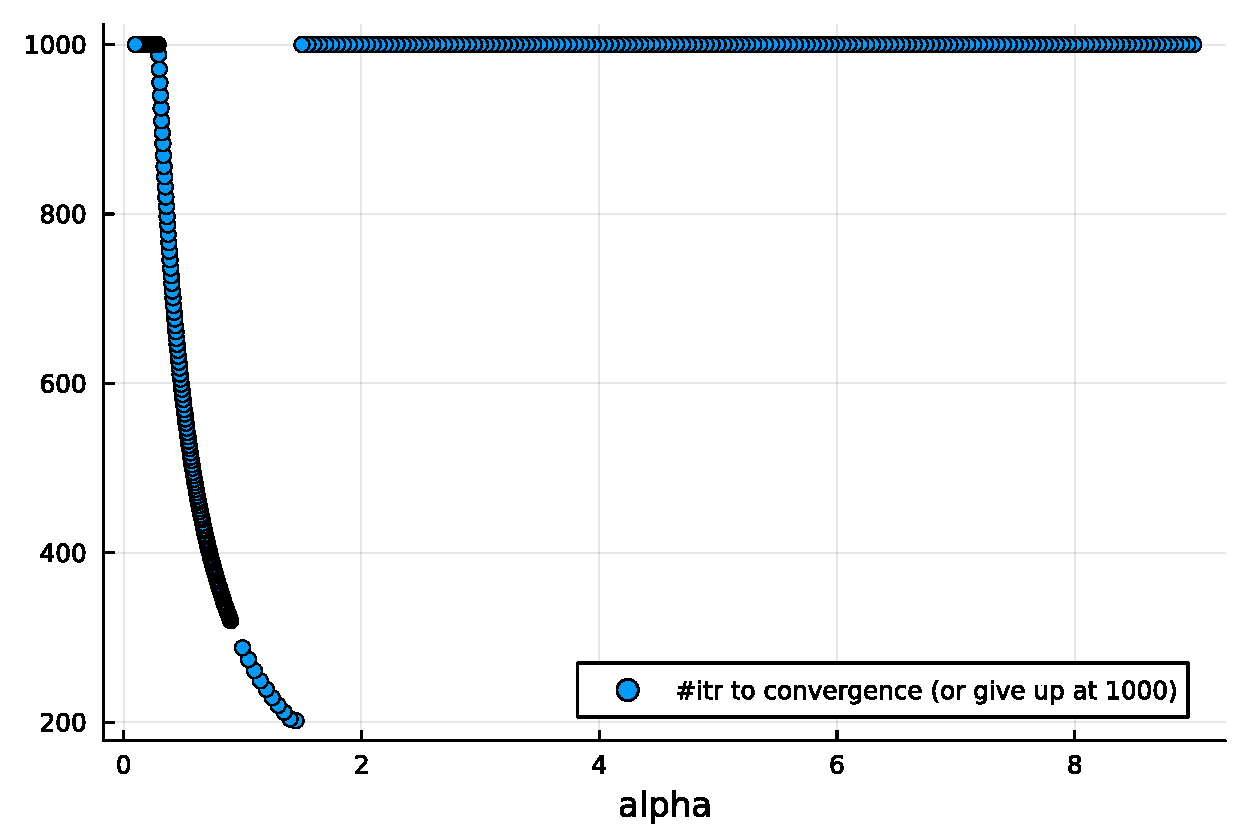
\includegraphics[width=.7\textwidth]{code/q4-1.pdf}
		\end{center}
	\item First, let's write out the linear equation we solved for in HW6:
		\begin{gather*}
			(\mI - \mT^T) \vx = \vy
		\end{gather*}
		Julia's solver gets us:
		\begin{gather*}
			\vx = (\mI - \mT^T)^{-1} \vy
		\end{gather*}
		We only want the 100th index. Using ideas from Q1-5, we bound $\rho(\mT^T) \leq \| \mT^T \|_\infty = 1$ as every row sums to 1 by definition.
		We know that for $\rho(\mT^T) < 1,~\lim_{\ell \rightarrow \infty} \sum^\ell_{k=0} (\mT^T)^{k} = (\mI - \mT^T)^{-1}$
		\begin{align*}
			\ell &= [(\mI - \mT^T)^{-1} \vy]_{100} \\
			\intertext{Using a one-hot encoded vector as selection:}
			&= \ve_{100} (\mI - \mT^T)^{-1} \vy \\
			\intertext{Applying Neumann Series:}
			&= \ve_{100} \sum^\infty_{k=0} (\mT^T)^k \vy \\
			\intertext{We can extract the first term:}
			&= \langle \ve_{100}, \vy \rangle + \ve_{100} \sum^\infty_{k=1} (\mT^T)^{k - 1} \mT^T \vy \\
			\intertext{Since $\vy_{100} = 0$, these are perpendicular vectors and nullify each other:}
			&= 0 + \ve_{100} \sum^\infty_{k=1} (\mT^T)^{k - 1} \mT^T \vy \\
			&= \sum^\infty_{k=1} \ve_{100} (\mT^T)^{k - 1} k \mT_{101, :} \\
			\intertext{Our result is a scalar, we can transpose the result and change nothing:}
			&= \sum^\infty_{k=1} k \mT^{k - 1} \mT_{:, 101} \ve_{100} \\
			\ell &= \sum^\infty_{k=1} k \left[\mT^{k - 1} \mT_{:, 101}\right]_{100} \\
		\end{align*}
		Which is the desired equivalent markovian computation.
\end{enumerate}

\newpage
\question
\hfill

Since we are working with a convex problem, any local minima is automatically a global minima. We can check for converge to the global optimizer not by comparing the residual but by checking for the gradient norm, as $\| \vg^{(k)} \| < \eps$ for some $\eps > 0$ is a valid convergence criteria. In this case, we'll set $\eps = 10^{-5}$.

\begin{lstlisting}
function steepest_descent(A, fv::Vector, T_max::Integer, tol::Number)
	x_hat = 1 * fv  # copy-by-value, not reference (https://stackoverflow.com/a/76109083/10671309)
	for itr in 1:T_max
		g_k = A * x_hat - fv   # matrix-vector product
		x_hat -= ((g_k' * g_k) / (g_k' * A * g_k)) * g_k   # extra (not-allowed) matrix product, included only for discussion; please see main implementation below
		if norm(g_k) < tol
			return (x_hat, itr)
		end
	end
	return (x_hat, T_max)
end

function steepest_descent(A, fv::Vector, T_max::Integer, alpha::Number, tol::Number)
	x_hat = 1 * fv  # copy-by-value, not reference (https://stackoverflow.com/a/76109083/10671309)
	for itr in 1:T_max
		g_k = A * x_hat - fv   # matrix-vector product
		x_hat -= alpha * g_k
		if norm(g_k) < tol
			return (x_hat, itr)
		end
	end
	return (x_hat, T_max)
end
\end{lstlisting}

Solving chutes and ladders using steepest descent with fixed step sizes results in a best-choice $\alpha = 1.4$ which solves it in 245 steps. Interestingly, with adaptive stepsizes, this took 257 iterations.

\begin{center}
	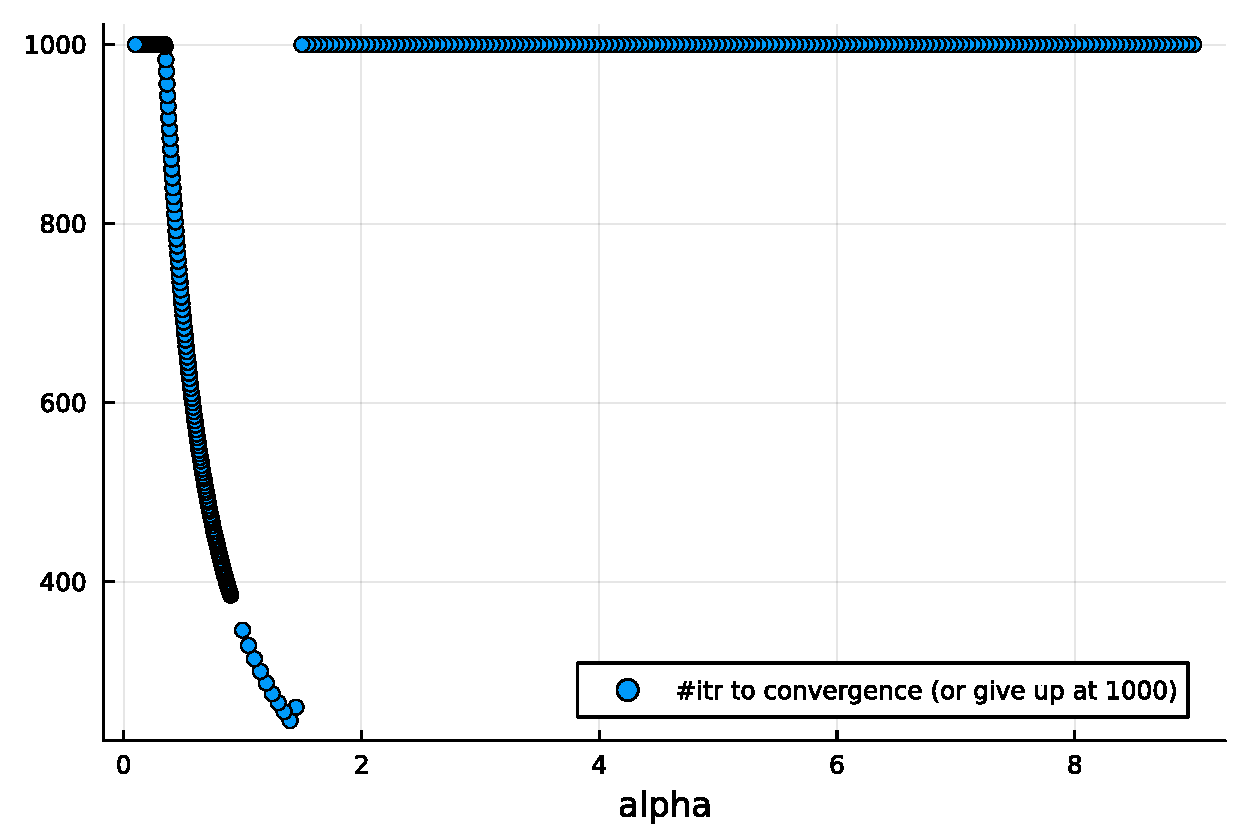
\includegraphics[width=.7\textwidth]{code/q5-1.pdf}
\end{center}

\newpage
\question
\hfill

\paragraph{Code}
\begin{lstlisting}
using SparseMatricesCSR, DelimitedFiles, LinearAlgebra, SparseArrays, Plots, Random

function partial_row_projection(rowptr, colval, nzval, row_idx, skip_col_idx, x)
	res = .0
	skip_val = 1

	for row_ptr in rowptr[row_idx]:(rowptr[row_idx+1]-1)  # only work on k non-zero entries
		if colval[row_ptr] != skip_col_idx
			res += x[colval[row_ptr]] * nzval[row_ptr]
		else
			skip_val = nzval[row_ptr]
		end
	end

	return res, skip_val
end

function random_coordinate_descent(rowptr, colval, nzval, y::Vector, T_max::Integer, tol::Number)
	x_hat = 1 * y  # copy-by-value, not reference (https://stackoverflow.com/a/76109083/10671309)
	for epoch in 1:T_max
		x_hat_new = similar(x_hat)

		for _ in 1:length(y)
			itr = rand(1:length(y))
			proj_val, skip_val = partial_row_projection(rowptr, colval, nzval, itr, itr, x_hat)
			x_hat_new[itr] = (y[itr] - proj_val) / skip_val
		end

		if norm(x_hat_new - x_hat) < tol
			return (x_hat, epoch * size(y)[1])
		end
		x_hat = 1 * x_hat_new
	end
	return (x_hat, T_max * size(y)[1])
end

function cyclic_coordinate_descent(rowptr, colval, nzval, y::Vector, T_max::Integer, tol::Number)
	x_hat = 1 * y  # copy-by-value, not reference (https://stackoverflow.com/a/76109083/10671309)
	for epoch in 1:T_max
		x_hat_new = similar(x_hat)

		for itr in 1:length(y)
			proj_val, skip_val = partial_row_projection(rowptr, colval, nzval, itr, itr, x_hat)
			x_hat_new[itr] = (y[itr] - proj_val) / skip_val
		end

		if norm(x_hat_new - x_hat) < tol
			return (x_hat, epoch * size(y)[1])
		end
		x_hat = 1 * x_hat_new
	end
	return (x_hat, T_max * size(y)[1])
end


coords = readdlm("chutes-and-ladders-coords.csv",',')
data = readdlm("chutes-and-ladders-matrix.csv",',')

xc = coords[:, 1]
yc = coords[:, 2]

TI = Int.(data[:,1])
TJ = Int.(data[:,2])
TV = data[:,3]
T = sparse(TI, TJ, TV, 101, 101)
A = SparseMatrixCSR(I - T')

is_dd = all((2 .* Array(diag(A)) - sum(A, dims=2)) .>= 0)
println("Is `A` diagonally dominant? ", is_dd)

y = ones(101)
y[100] = 0

Random.seed!(0)
T_max = 1000000
tol = 1e-10

x_oracle = A\y

x_r, itr_r = random_coordinate_descent(A.rowptr, A.colval, A.nzval, y, T_max, tol)
x_c, itr_c = cyclic_coordinate_descent(A.rowptr, A.colval, A.nzval, y, T_max, tol)

println(norm(x_oracle - x_r))
println(norm(x_oracle - x_c))
\end{lstlisting}

\paragraph{Output}

\begin{lstlisting}
Is `A` diagonally dominant? true
2.4148946143466656e-9
2.4148946143466656e-9
\end{lstlisting}

The random case depends on the mercy of the gods and is {\it much} slower to converge as a result:
\begin{lstlisting}
julia> itr_r
20094152

julia> itr_c
63024
\end{lstlisting}

\newpage
\question
\hfill

\begin{lstlisting}
function gen_coord_descent(A, y::Vector, T_max::Integer, tol::Number, n_coords::Integer)
	x_hat = 1 * y  # copy-by-value, not reference (https://stackoverflow.com/a/76109083/10671309)
	for itr in 1:T_max
		g_k = A * x_hat - y   # matrix-vector product
		update = ((g_k' * g_k) / (g_k' * A * g_k)) * g_k

		for start in 1:n_coords:length(y)-n_coords
			for coord in start:start+n_coords
				x_hat[coord] -= update[coord]
			end
		end

		if norm(g_k) < tol
			return (x_hat, itr * length(y) / n_coords)
		end
	end
	return (x_hat, T_max * length(y) / n_coords)
end
\end{lstlisting}

\newpage
\question
\hfill

\paragraph{Code}
\begin{lstlisting}
include("q1.jl")
include("q5.jl")
include("q6.jl")

# 2d laplacian
n = 40
A, y = laplacian(n, (x, y) -> 1)

A = SparseMatrixCSR(A[4n+1:end,4n+1:end])
y = y[4n+1:end]

# chutes and ladders
coords = readdlm("chutes-and-ladders-coords.csv",',')
data = readdlm("chutes-and-ladders-matrix.csv",',')

xc = coords[:, 1]
yc = coords[:, 2]

TI = Int.(data[:,1])
TJ = Int.(data[:,2])
TV = data[:,3]
T = sparse(TI, TJ, TV, 101, 101)
A = SparseMatrixCSR(I - T')

y = ones(101)
y[100] = 0


T_max = 1000
alpha = 1.4
tol = 1e-4

tols = []
works_stpd = []
works_coord = []
for tol_pow in 1:4
	for tol_coeff in 9:-.1:1
		local tol = tol_coeff * 10^(-1. * tol_pow)
		local x_stpd, itr_stpd = steepest_descent(A, y, T_max, tol)
		local work_stpd = itr_stpd * nnz(A)

		local x_coord, itr_coord = cyclic_coordinate_descent(A.rowptr, A.colval, A.nzval, y, T_max, tol)
		local work_coord = itr_coord / length(y) * nnz(A)

		push!(tols, tol)
		push!(works_stpd, work_stpd)
		push!(works_coord, work_coord)
	end
end

p = scatter(tols, works_stpd, label="Steepest Descent")
p = scatter!(tols, works_coord, label="Coordinate Descent", xlabel="tolerance", ylabel="work", yscale=:log10, xscale=:log10)
p = xflip!(true)
\end{lstlisting}

\begin{enumerate}[label=\arabic*.]
	\item For the 2D Laplacian, steepest descent does well in the start (when tolerances are high) but as we up the ante coordinate descent comes out a clear winner.
		\begin{center}
			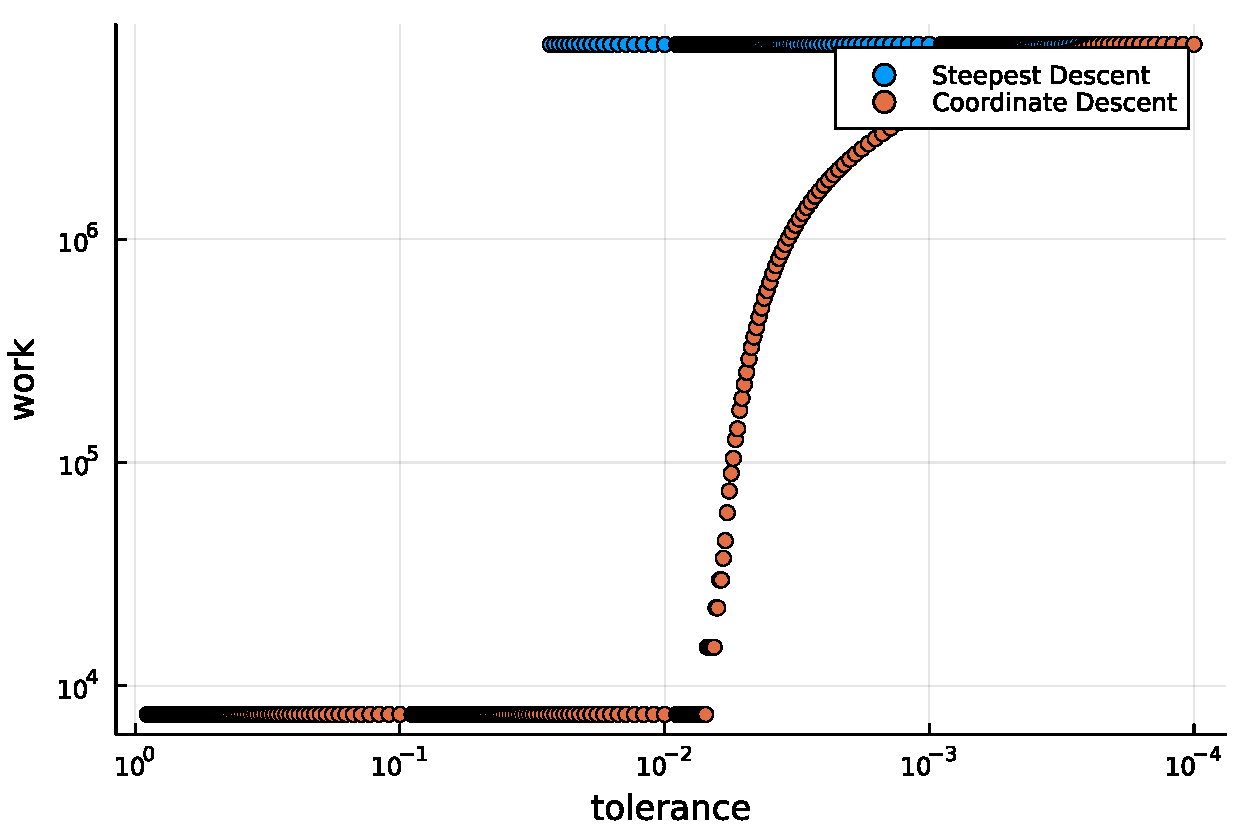
\includegraphics[width=.7\textwidth]{code/q8-2.pdf}
		\end{center}
		\begin{table}[]
			\centering
			\begin{tabular}{@{}lll@{}}
				\toprule
				Tolerance             & Work by Steepest Descent & Work by Coordinate Descent \\ \midrule
				0.9                   & 7449                     & 7449                       \\
				0.65                  & 7449                     & 7449                       \\
				0.4                   & 7449                     & 7449                       \\
				0.15000000000000002   & 7449                     & 7449                       \\
				0.07100000000000001   & 7449                     & 7449                       \\
				0.046000000000000006  & 7449                     & 7449                       \\
				0.021000000000000005  & -                        & 7449                       \\
				0.0077                & -                        & 7449                       \\
				0.005200000000000001  & -                        & 171327                     \\
				0.0027                & -                        & 1.556841e6                 \\
				0.0008300000000000001 & -                        & 4.402359e6                 \\
				0.00058               & -                        & 5.266443e6                 \\
				0.00033               & -                        & 6.62961e6                  \\
				0.0001                & -                        & 7.449e6					  \\
				\bottomrule
			\end{tabular}
		\end{table}
	\item For chutes and ladders, steepest descent outperforms coordinate descent by across every convergence threshold.
		\begin{center}
			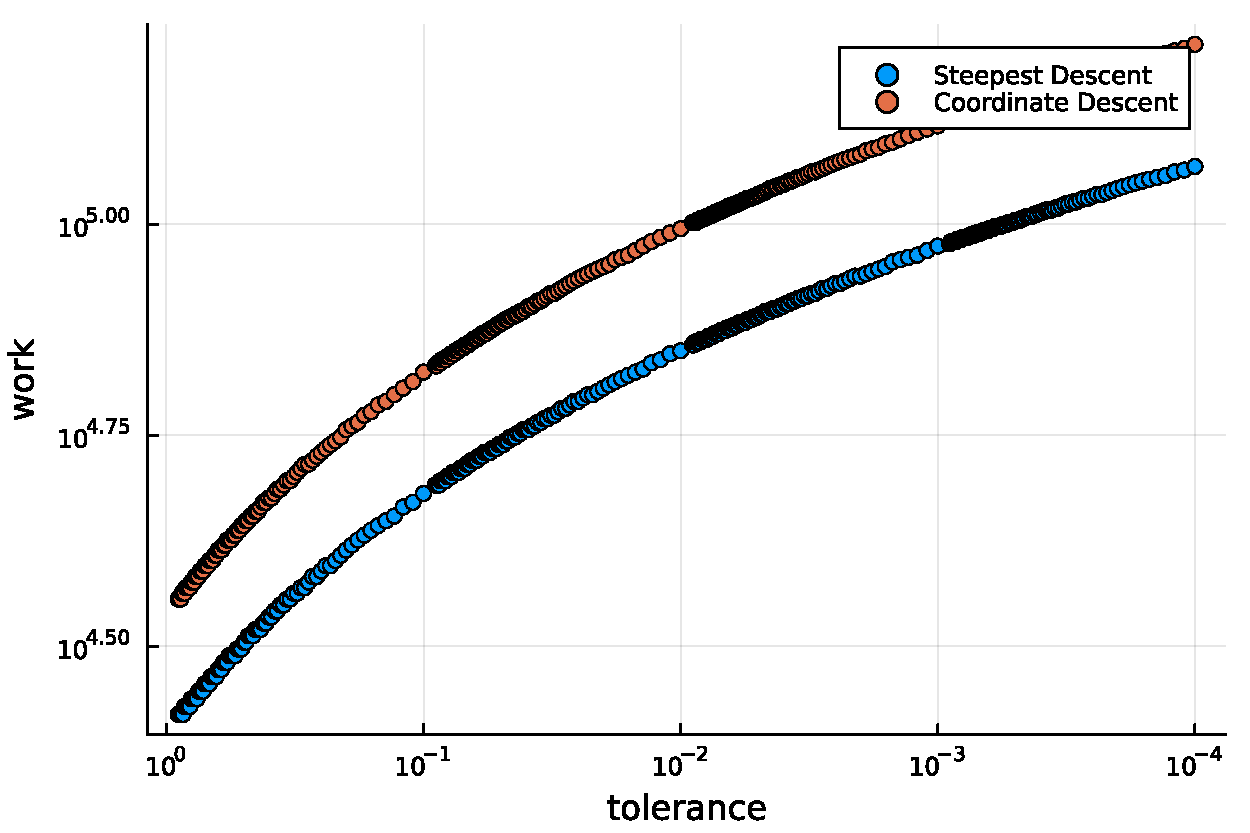
\includegraphics[width=.7\textwidth]{code/q8-1.pdf}
		\end{center}
		For the table, we sample from various tolerance levels to prevent overcrowding.
		\begin{table}[]
			\centering
			\begin{tabular}{@{}lll@{}}
				\toprule
				Tolerance             & Work by Steepest Descent & Work by Coordinate Descent \\ \midrule
				0.9                   & 26266                    & 35973                      \\
				0.65                  & 29121                    & 40541                      \\
				0.4                   & 34260                    & 47393                      \\
				0.15000000000000002   & 43967                    & 61097                      \\
				0.07100000000000001   & 51390                    & 71375                      \\
				0.046000000000000006  & 55958                    & 77656                      \\
				0.021000000000000005  & 63381                    & 88505                      \\
				0.0077                & 73659                    & 102209                     \\
				0.005200000000000001  & 77656                    & 107919                     \\
				0.0027                & 83937                    & 117055                     \\
				0.0008300000000000001 & 95928                    & 133614                     \\
				0.00058               & 99354                    & 138753                     \\
				0.00033               & 105064                   & 146176                     \\
				0.0001                & 117055                   & 163306                     \\
				\bottomrule 
			\end{tabular}
		\end{table}
\end{enumerate}

\newpage
\question
\hfill

We have the following linear system:
\begin{gather*}
	\mA \vx = \vb \iff (\mD + \mN) \vx = \vb
\end{gather*}
We also have diagonal dominance, where for some $\gamma < 1$ it holds that:
\begin{gather*}
	\| \mA \vx - \mD \vx \| \leq \gamma \| \mD \vx \|
\end{gather*}
We update elements elementwise:
\begin{gather*}
	\vx^{(k)}_i = \frac{1}{\mA_{i,i}} (\vb_i - \langle \mN_{i, :}, \vx^{(k - 1)} \rangle)
\end{gather*}
Which can be rewritten for the entire guess $\vx^{(k)}$ as:
\begin{gather*}
	\vx^{(k)} = \mD^{-1} (\vb - \mN \vx^{(k - 1)})
\end{gather*}
% 
% T.P.T.
% \begin{gather*}
% 	\forall \eps > 0~\exists k \in \mathbb{N} : \| \mA \vx^{(k)} - \vb \| < \eps \\ \\
% \end{gather*}
Since $\mA$ is diagonally dominant, and diagonal dominance implies positive definiteness (we used this fact in the programming questions), we can approach this problem through the lens of convex minimization:
\begin{gather*}
	\min_{\vx} \frac{1}{2} \vx^T \mA \vx - \vx^T \vb
\end{gather*}
Under this formulation, we can show that the update at each iteration is the gradient scaled coordinate-wise:
\begin{align*}
	\vx^{(k)} &= \mD^{-1} (\vb - \mN \vx^{(k - 1)}) \\
	&= \mD^{-1} (\vb - (\mA - \mD) \vx^{(k - 1)}) \\
	&= \mD^{-1} \vb - \mD^{-1} \mA \vx^{(k-1)} + \mD^{-1} \mD \vx^{(k - 1)} \\
	\vx^{(k)} &= \vx^{(k - 1)} - \underbrace{\mD^{-1}}_{\text{step size}} \underbrace{(\mA \vx^{(k-1)} - \vb)}_{\vg^{(k - 1)}}
\end{align*}
A sufficient condition for the convergence of steepest descent is $\alpha < \nicefrac{2}{\rho(\mA)}$, for the elementwise case we will prove that $\mD^{-1}_{ii} < \nicefrac{2}{\rho(\mA)}$ for every index $i$. By diagonal dominance, we have that:
\begin{gather*}
	\rho(\mA) \leq \| \mA \|_{\infty} = \max_{i} \sum_{j} |\mA_{i,j}| < 2 \max_{i}(\mD_{i,i}) \\
	\therefore \frac{2}{\rho(\mA)} > \frac{1}{\max_i \mD_{i,i}} = \left(\max_i \mD_{i,i}\right)^{-1} 
\end{gather*}
Since we have proven the desired statement for the max, this also follows for any $i$, and through this equivalence we have that Jacobi does converge.

% Checking error:
% \begin{align*}
% 	\vx^{(k)} - \vx &= \vx^{(0)} + \left(\mD^{-1}\right)^k \sum^{k}_{i=1} (\vb - \mA \vx^{(i)}) - \vb - \vx
% \end{align*}
% Checking error:
% \begin{align*}
% 	\| \mA \vx^{(k)} - \vb \| &= \left\| (\mD + \mN) \vx^{(k)} - \vb \right\| \\
% 	&= \left\| \mD \vx^{(k)} + \mN \vx^{(k)} - \vb \right\| \\
% \end{align*}
% Checking error:
% \begin{align*}
% 	\| \mA \vx^{(k)} - \vb \| &= \left\| \mA \left( \vx^{(k - 1)} + \mD^{-1} (\vb - \mA \vx^{(k-1)}) \right) - \vb \right\| \\
% 	&= \left\| \mA \left( \vx^{(k - 2)} + \mD^{-1} (\vb - \mA \vx^{(k-2)}) + \mD^{-1} (\vb - \mA \vx^{(k-1)}) \right) - \vb \right\| \\
% 	&= \left\| \mA \left( \vx^{(0)} + \sum^{k}_{i=1} \mD^{-1} (\vb - \mA \vx^{(i)}) \right) - \vb \right\| \\
% 	&= \left\| \mA \left( \vx^{(0)} + \left(\mD^{-1}\right)^k \sum^{k}_{i=1} (\vb - \mA \vx^{(i)}) \right) - \vb \right\| \\
% 	&= \left\| \left( \mA \left(\mD^{-1}\right)^k \sum^{k}_{i=1} (\vb - \mA \vx^{(i)}) \right) - \mA \vx^{(0)} \vb \right\| \\
% \end{align*}

\newpage
\question
\hfill

In the linear algebraic approximation, we can decompose viral spread at time $t$ with the following equation:
\begin{equation*}
	\vx^{(t)} = \rho \mA \vx^{(t-1)} = (\rho \mA)^t \vx^{(0)} =(\mV \Lambda^t \mV^T) \vx^{(0)}
\end{equation*}
If the largest eigenvalue of $\rho \mA > 1$, as $t \rightarrow \infty$ the probability of infection diverges. In contrast for a maximum eigenvalue $< 1$, spread as timesteps progress tends to 0, thus our approximate model (calculating cumulative probability) reduces to a convergent Nuemann series, which depends on the spectral radius to guarantee convergence and find a steady state for this suitable regime.

\end{questions}
\end{document}
